%Authors guidlines: http://royalsocietypublishing.org/instructions-authors
% 2500 words max (includes the title page, abstract, references, acknowledgements and figure/table legends)
% current version is around 3700. I think a big cut down can be done on the references.
% We allow a maximum of 4 displays, only 2 of which can be figures.

\documentclass[12pt,letterpaper]{article}


%Packages
\usepackage{pdflscape}
\usepackage{fixltx2e}
\usepackage{textcomp}
\usepackage{fullpage}
\usepackage{float}
\usepackage{latexsym}
\usepackage{url}
\usepackage{epsfig}
\usepackage{graphicx}
\usepackage{amssymb}
\usepackage{amsmath}
\usepackage{bm}
\usepackage{array}
%\usepackage{mhchem}
\usepackage{ifthen}
\usepackage{caption}
\usepackage{hyperref}
\usepackage{amsthm}
\usepackage{amstext}
\usepackage{enumerate}
\usepackage[osf]{mathpazo}
\usepackage{dcolumn}
\usepackage{lineno}
\usepackage{longtable}

\pagenumbering{arabic}

\newcolumntype{L}[1]{>{\raggedright\let\newline\\\arraybackslash\hspace{0pt}}m{#1}}
\newcolumntype{C}[1]{>{\centering\let\newline\\\arraybackslash\hspace{0pt}}m{#1}}
\newcolumntype{R}[1]{>{\raggedleft\let\newline\\\arraybackslash\hspace{0pt}}m{#1}}

%Pagination style and stuff % NC: Note that these are all syst biol specific.
\linespread{2}
\raggedright
\setlength{\parindent}{0.5in}
\setcounter{secnumdepth}{0} 
\renewcommand{\section}[1]{%
\bigskip
\begin{center}
\begin{Large}
\normalfont\scshape #1
\medskip
\end{Large}
\end{center}}
\renewcommand{\subsection}[1]{%
\bigskip
\begin{center}
\begin{large}
\normalfont\itshape #1
\end{large}
\end{center}}
\renewcommand{\subsubsection}[1]{%
\vspace{2ex}
\noindent
\textit{#1.}---}
\renewcommand{\tableofcontents}{}
%\bibpunct{(}{)}{;}{a}{}{,}

%---------------------------------------------
%
%       START
%
%---------------------------------------------

\begin{document}

%Running head
\begin{flushright}
Version dated: \today
\end{flushright}

\bigskip
\medskip
\begin{center}

\noindent{\Large \bf How Information Kills: the Case of Foraging Seabirds} 

\bigskip

\noindent {\normalsize \sc Adam Kane$^1$$^,$$^*$}\\ %and John Quinn$^1$}\\
\noindent {\small \it 
$^1$Biological, Earth and Environmental Sciences, University College Cork, Cork, Ireland}\\

\end{center}
\medskip
\noindent{*\bf Corresponding author.} \textit{adam.kane@ucc.ie}\\  
\vspace{1in}

%Line numbering
\modulolinenumbers[1]
\linenumbers

%---------------------------------------------
%
%       ABSTRACT
%
%---------------------------------------------
\newpage
\begin{abstract}
%\section{abstract} : Just put this here as it then separates this for the word count
Animals frequently take cues from other individuals to improve their chances of finding food. This is a common behaviour in seabirds that search for patchily distributed fish shoals. However, information sharing might also pose a danger in that individuals may be attracted to an animal who is foraging in a dangerous area. Potential dangers at sea are numerous and include, oil slicks, fishing equipment, and energy infrastructure. Here, we create an agent-based model to investigate whether or not shared information can endanger foraging seabirds. We consider three levels: those who rely on personal information, those who also avail of local enhancement and those who can detect cues at the colony. Our results suggest that as a bird takes in ever more social cues, its risk of death increases. Our work should be of interest to conservationists involved in drawing up risk indices for separate species; information use is one trait that has been neglected to date. 

\end{abstract}

\noindent Key words: information use, social foraging, energy infrastructure, conservation, oil, fisheries\\


\vspace{1.5in}

%---------------------------------------------
%
%       INTRODUCTION
%
%---------------------------------------------
\newpage 
\section{Introduction}
A great benefit of group living is the ability to garner information about your environment from those around you \cite{dall2005information}. This is especially useful to a foraging animal who can hone in on other individuals who have successfully discovered food. This typically manifests as a local enhancement effect such that the efforts of one animal are conspicuous enough to draw the attention of another \cite{KaneVul,buckley1997spatial}. Information on resource location is especially useful in areas with patchily distributed resources, for instance, at sea with shoals of fish \cite{thompson2001long}. Here, a diving bird represents a clear signal to others that it has found food. This signal is inadvertent so that there is no obvious way for the finder to mask its discovery. Moreover, there is a mounting body of evidence from tracking studies to suggest that seabirds also use colonies and the areas surrounding them as information centres \cite{ward1973importance, burger1997arrival, weimerskirch2010use,wakefield2013space}. This behaviour occurs both within and among species. In this case, naive birds are able to distinguish between successful and unsuccessful foragers at these 'centres' and so can follow them back out to sea directly or fly in the direction from which they came. 

However, these behaviours may in fact imperil animals in certain situations \cite{giraldeau2002potential}. Consider seabirds foraging near to wind turbines, oil slicks, wave energy devices, fishing vessels etc. By following a successful forager to a site where such structures or vehicles are active may endanger them to lethal collisions. Similarly for birds using their colonies as information centres who may be following a previously successful forager to their death. Thus, it is our hypothesis that differential information use can affect the probability a bird enters a dangerous area. With the booming renewable energy industry, ongoing fisheries and the continuing risk of oil spills the world over, there are many risks to seabirds foraging over the oceans \cite{furness2013assessing,williams1995method}.  





%---------------------------------------------
%
%       METHODS
%
%---------------------------------------------
\section{Materials and Methods}
We built an agent-based model implemented in NetLogo version 5.2.1 \cite{tisue2004netlogo} to test the effect information use can have on the survival of foraging birds. The simulation space has a colony of 100 birds at its centre and a number of fish shoals that move around the sea at a set rate but can be disturbed if enough birds feed on them to move around the habitat more quickly. The environment consists of 100 x 100 patches. Randomly located throughout the environment are 40 structures with which the birds can collide and be killed while feeding. 

There are 3 types of birds who are differentiated according to how they use information. Firstly, nulls rely entirely on personal information. Once they detect a fish patch in their visual radius they move towards it, feed and fly back to the colony. They will fly back to this patch on the next foraging occasion. Gulls add another level of complexity by using local enhancement, in addition to personal information. This is realised by allowing the gulls to spot fish patches that are being fed upon by other birds. The gulls can detect this at a longer range than they can detect undisturbed food. This is realistic because a diving bird is a more conspicuous target than a fish shoal beneath the water. Finally, gannets, while using personal and local enhancement information, also use their colony as an information centre. In this instance, unsuccessful foragers will follow a successful one back to sea. All 3 bird types have a set energy that is depleted as they forage. Once this reaches 0 they have to return to the colony. The birds all have an equal turning rate and flight speed. 

We ran models for each of these birds types in turn i.e. only nulls for a given simulation. Each simulation was ran 100 times. The stop condition was reached once 50\% of the birds had died. We also ran an analysis to determine if increased information sharing improved foraging efficiency in the first place without any of the dangerous structures present. The stop condition in this case was achieved once 75\% of the birds had found food. All of the data were extracted and analysed using R \cite{RCran} and the R-NetLogo interface RNetLogo \cite{thiele2014r}.  
%---------------------------------------------
%
%       RESULTS
%
%---------------------------------------------


\section{Results}
Our results show a significant effect of information use on the survival of foraging seabirds (ANOVA: F-value = 228.8, p \textless 0.001, $\eta^2$ = 0.606; Tukey post hoc test showed that all groups differed significantly, p \textless 0.001). As we moved in complexity from personal information users to local enhancement users and finally onto those who could glean information around their colonies, the risk of death increased. In figure \ref{info.diff} we can see a box plot of the log\textsubscript{10} of time until 50 \% mortality against information use which illustrates this finding. We also showed foraging efficiency improved with increased information sharing (ANOVA: F-value = 581.5, p \textless 0.001, $\eta^2$ = 0.796; Tukey post hoc test showed that all groups differed significantly, p \textless 0.001). 

\begin{table}[]
\centering
\caption{Summary statistics for the time until 50 \% mortality for the three types of information users in the model. SD = standard deviation.}
\label{my-label}
\begin{tabular}{lll}
\hline 
\textbf{Information use} & \textbf{Mean} & \textbf{SD} \\
\hline 
personal information     & 46257         & 49846       \\
local enhancement   & 18433         & 11500       \\ 
information transfer      & 6693          & 7848       \\ 
\hline 

\end{tabular}
\end{table}



\begin{figure}[H]
\centering
    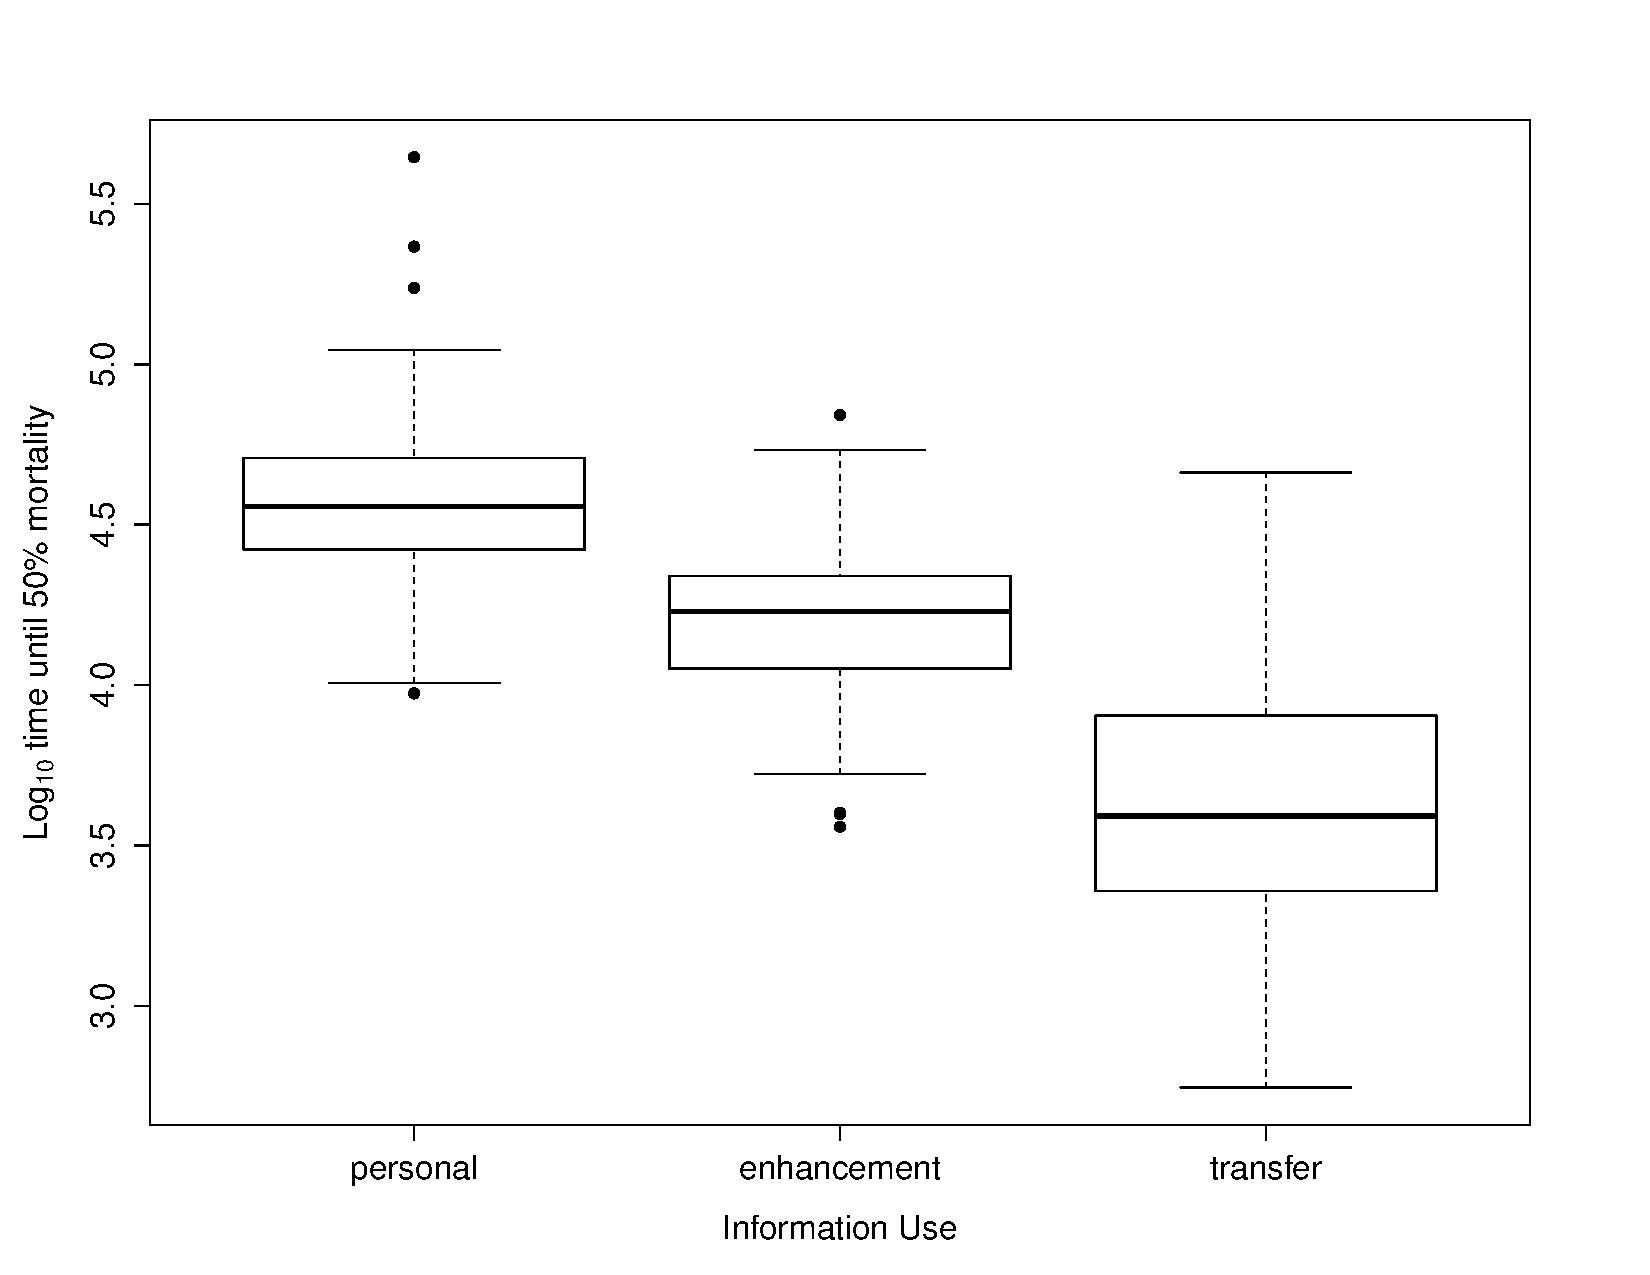
\includegraphics[keepaspectratio, totalheight=0.6 \textheight]{figure.pdf}
\caption{Time until mortality as a function of information use}
\label{info.diff}
\end{figure}



%---------------------------------------------
%
%       DISCUSSION
%
%---------------------------------------------

\section{Discussion}
The pattern we found should be intuitive to understand. Birds relying on their memory pay no heed to any other foraging animal. But once social information starts to be used there is a black hole effect in that the behaviour of one individual can drag others to a dangerous patch in the case of local enhancement. And in the worst case scenario, a successful forager can attract many birds from the colony to a site where they might be killed. 

The results of this modelling approach have empirical support. Weimerskirch and colleagues found a difference in information use between Peruvian boobies (\textit{Sula variegata}) and Guanay cormorants (\textit{Phalacrocorax bougainvillii}) \cite{weimerskirch2010use}. The former relied mainly on personal information while the latter formed rafts away from the colony which acted as information centres. This difference may be the cause of the differential trend in their respective populations whereby the cormorants have suffered a decline but the boobies have remained stable. Aside from cormorants, there is evidence of information transfer in other seabirds including, Northern Gannets \cite{wakefield2013space}, Common Guillemots \cite{burger1997arrival} and Albatrosses \cite{weimerskirch2010use} so the consequences of this behaviour should be both a cause for concern and a point of interest for conservationists. In the case of fisheries, the creation of fish bycatch often attracts birds but this industry is well known for endangering these same birds. For instance, fishing gear like nets and hooks can entangle or maim the birds ultimately killing them \cite{tasker2000impacts}. The addition of this extra risk caused by information use means certain species are even more at risk when they avail of fisheries bycatch. Similarly, the literature on the dangers of renewable energy infrastructure to seabirds is on the rise \cite{furness2013assessing}. Specific traits such flight height can influence risk of mortality. Again, social information use represents another important trait to consider. Outside of seabirds there are many other species that may be affected in similar ways. For instance, vultures are colonial birds that use inter and intra specific information while searching for patchily distributed carrion \cite{KaneVul}. 

Finally, the results also speak to the benefits of modelling. Our approach afforded us the flexibility to vary information use while keeping every other behaviour constant. Agent-based models have a lot of value when considering spatially explicit issues. 


%Biology letters various stuff
\section{Ethics statement}
N/A
\section{Data accessibility statement}
All data and analysis code is available on GitHub (\url{https://github.com/kanead}).
\section{Authors' Contributions}
All authors approved the final version of the manuscript.
%A.K. conceived and designed the experiments. A.K. performed the experiments and analysed the data. A.K. and J.Q. contributed to the writing of the manuscript. 
\section{Competing Interests}
We have no competing interests.
\section{Acknowledgments}
We thank Thomas Guillerme, Deirdre McClean
\section{Funding statement}
This work was funded by an Irish Research Council Postdoctoral Fellowship.

\bibliographystyle{vancouver}
\bibliography{References}

%END
\end{document}
